%prezentacja do pracy inżynierskiej (c) Kamil Strzempowicz
\documentclass{prezentacja}
%\usepackage{polski}
\usepackage{mathtools}
\usepackage{color}
\usepackage{graphicx}
\usepackage{transparent}
\usepackage{wrapfig}

%hyperref musi być ostatnie
%\usepackage[hidelinks]{hyperref}

%\mathtoolsset{showonlyrefs}

%%%%%%%%%%%%%%%%%%%%%%%
%%% Podstawowe info %%%
%%%%%%%%%%%%%%%%%%%%%%%

\title{Strategia Just in Time w systemach produkcyjnych\\ - analiza struktury gniazdowej dla heurystyk FIFO i LIFO}
\promotor{dr inż. Waldemar Grzechca}
\autor{Kamil Strzempowicz}
\author{Kamil Strzempowicz}
\rodzPracy{Prezentacja projektu inżynierskiego}
\kierunek{Automatyka i Robotyka}
\institute{Wydział Automatyki, Elektroniki i Informatyki}
\usetheme{lined} %motyw
\usecolortheme{dove}


\setlength\intextsep{0pt}
\setlength{\wrapoverhang}{\marginparwidth}
\addtolength{\wrapoverhang}{\marginparsep}
%%%%%%%%%%%%%%%%%%%%%%%%%%%%%%%%%
%%% początek właściwej treści %%%
%%%%%%%%%%%%%%%%%%%%%%%%%%%%%%%%%

\begin{document}

\begin{frame}
    \StronaTyt
\end{frame}
\begin{frame}
    \frametitle{Spis tresci}
    \tableofcontents
\end{frame}
\section{Wstęp teoretyczny}
\begin{frame}
    
    \begin{wrapfigure}{R}{.4\linewidth}
        \vspace{-110pt}
        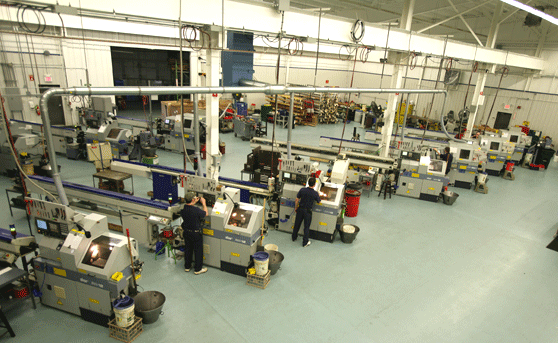
\includegraphics[width=\linewidth, keepaspectratio=true]{./obrazki/job-shop}
        \caption{ Przykład systemu gniazdowego\cite{swiss}}
    \end{wrapfigure}
    
    \frametitle{Systemy gniazdowe}
    \vspace{60pt}
    Najczęściej wykorzystywane do pojedynczych zamówień, bądź krótkich serii. Takie systemy zwykle zmieniają swoje zastosowanie po zakończeniu każdego zlecenia. Zlecenie składa się ze skończonej liczby zadań, a~każde z~nich wymaga przeprowadzenia zestawu operacji na maszynach w~ustalonym porządku, innym dla każdego zadania.
    
   

\end{frame}
\begin{frame}
    \frametitle{Strategia Just in Time}
    Zadanie powinno być ukończone możliwie blisko swojego terminu zakończenia (due date) jak to tylko możliwe. Zbyt wczesne zakończenie zadania pociąga za sobą koszty utrzymania, takie jak magazynowania czy ubezpieczenia. Z~drugiej jednak strony spóźnione zlecenie często skutkuje karami umownymi czy nadszarpnięciem reputacji przedsiębiorstwa \cite{genetyczne}.

    Na potrzeby tej pracy wybrano następujące funkcje matematycznie opisujące dostosowanie uszeregowania do strategii JIT:
\small{
    \begin{equation}
        \sqrt{\sum e_j^2 + \sum l_j^2}
        \label{eq:w1}
    \end{equation}
    \begin{equation}
        \alpha*\sum e_j + \beta*\sum l_j
        \label{eq:w2}
    \end{equation}
}
\footnotesize{
    \begin{tabular}{r l}    
    \(e_j\) & przedwczesność j-tego zadania, \\
    \(l_j\) & spóźnienie j-tego zadania, \\
    \(\alpha, \beta\) & wagi przedwczesności i~spóźnienia.
    \end{tabular}
}
\end{frame}
\section{Program kSzereg}
\begin{frame}   
    \begin{wrapfigure}{r}{.4\linewidth}
        \vspace{-75pt}
        
\includegraphics[width=\linewidth, keepaspectratio=true]{./obrazki/QtLogo}
      %  \caption{ Przykład systemu gniazdowego\cite{swiss}}
    \end{wrapfigure}
    
    \frametitle{Program kSzereg}
    Program kSzereg został napisany w~C++ na potrzeby tej pracy dyplomowej. Umożliwia on przeprowadzenie szeregowania zadań w~systemie wytwarzania gniazdowego na podstawie heurystyki \emph{First In First Out} bądź \emph{Last In First Out}. 
    
    Wprowadzanie danych odbywa się za pośrednictwem graficznego interface'u opartego o~framework Qt.
\end{frame}
\def\ofset{1.4cm}
\hspace{-\ofset}
\begin{frame}
    \frametitle{\hspace{\ofset}Główne okno}
    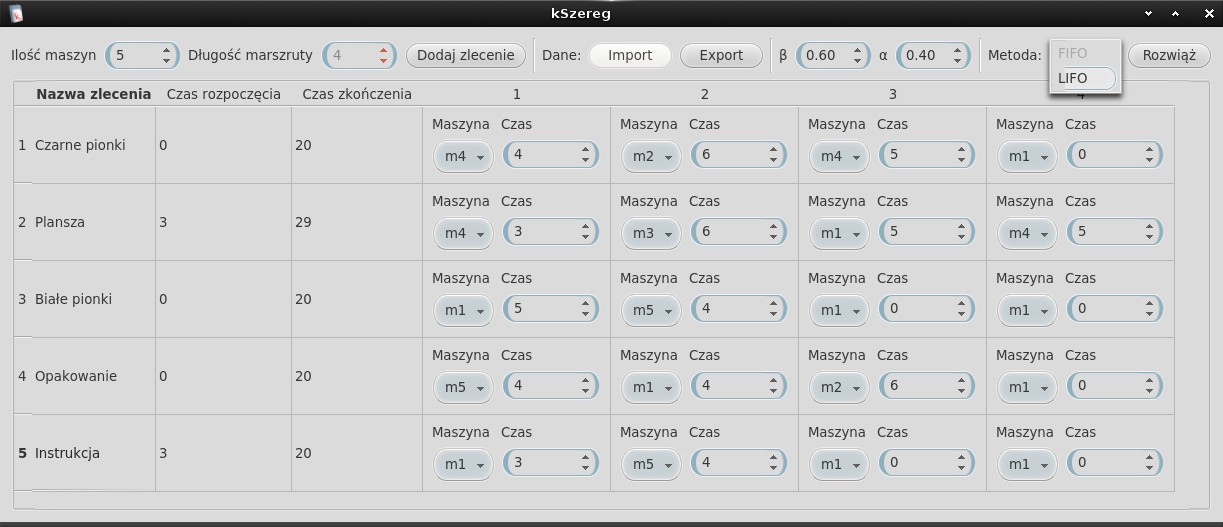
\includegraphics[width=\paperwidth-.45cm, keepaspectratio=true]{./obrazki/s1}
\end{frame}
\begin{frame}
    \frametitle{Okno rozwiązania}
    \begin{figure}[htb]
        \centering
        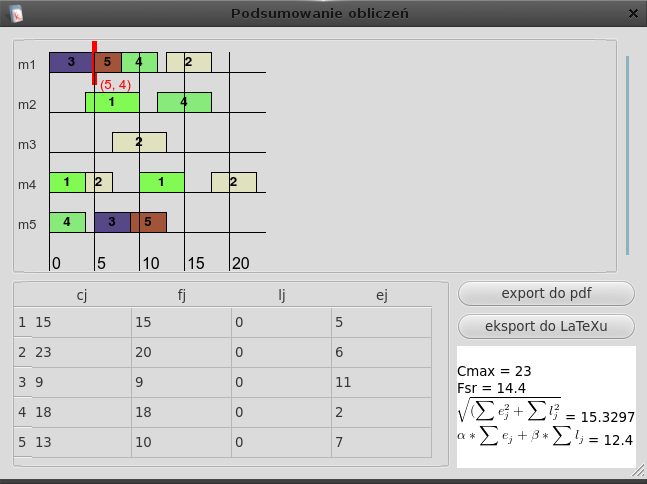
\includegraphics[height=.8\textheight, keepaspectratio=true]{./obrazki/s2}
    \end{figure}    
\end{frame}
\begin{frame}
    \frametitle{Linia poleceń}
    \begin{figure}[htb]
        \centering
        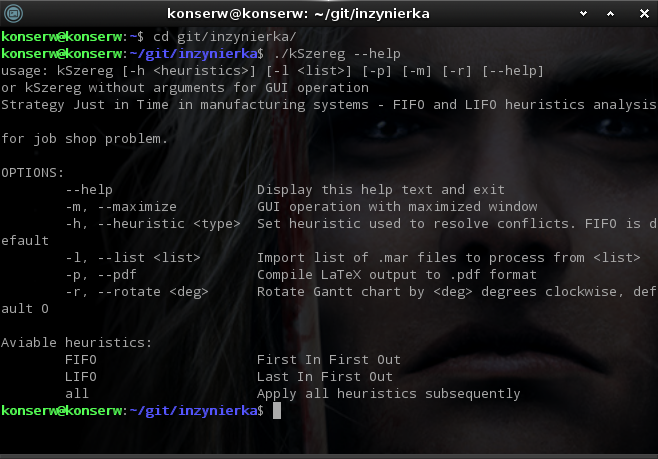
\includegraphics[height=.8\textheight, keepaspectratio=true]{./obrazki/s3}
    \end{figure}  
\end{frame}
\section{Rozpatrywane zlecenia}
\begin{frame}
    \frametitle{Rozpatrywane zlecene}
    
    
\end{frame}
\section{Wnioski}
\begin{frame}
    
\end{frame}
\section{Literatura}
\begin{thebibliography}{1}
\begin{frame}
\bibitem{swiss}
\emph{Strona internetowa firmy Swissturn},
Źródło: \url{http://www.swissturn.com} [dostęp:~21.01.2013]

\bibitem{genetyczne}
Rodolfo Pereira Araujo, André Gustavo dos Santos, José Elias Cláudio Arroyo,
\emph{Genetic Algorithm and Local Search for Just-in-Time Job–Shop Scheduling},
2009 IEEE Congress on Evolutionary Computation (CEC 2009)
\end{frame}
\end{thebibliography}
\end{document}        
